\begin{center}
\begin{sideways}%[htbp]
	\begin{minipage}{1.3\textwidth}
		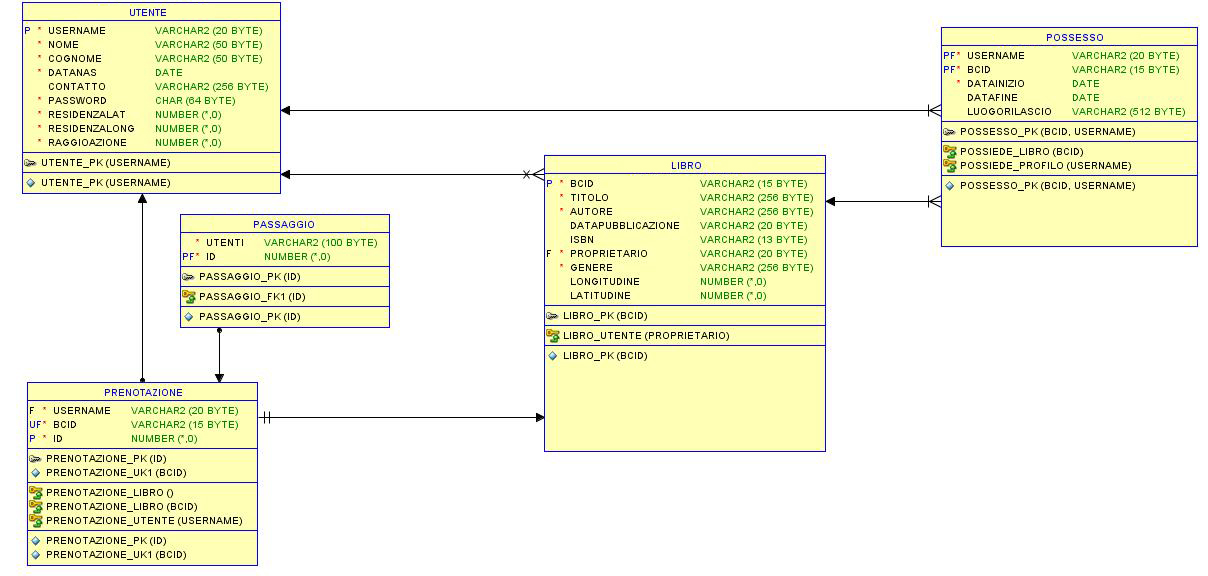
\includegraphics[width=\linewidth,keepaspectratio]{Immagini/db_schema.jpg}
		\captionof{figure}{Modello del databse}
		\vspace{0.2cm}
		\label{fig:xx}
	\end{minipage}
\end{sideways}
\end{center}

La figura 3.3 rappresenta il modello logico del database, le cui entità sono:
\begin{itemize}
	\item \textbf{Utente} : contiene tutti i dati relativi all'utenza registata, ogni utente è identificato da uno \textit{username} univoco;
	\item \textbf{Libro} : contiene tutti i libri presenti nel sistema, ognuno dei quali è identificato da un BCID generato univocamente;
	\item \textbf{Prenotazione} : rappreseta la relazione N:N tra Utente e Libro;
	\item \textbf{Passaggio} : contiene la sequenza di utenti che dovrebbero partecipare in maniera attiva alla prenotazione indicata dalla PK della tabella stessa;
	\item \textbf{Possesso} : questa tabella rappresenta i libri attualmente in possesso dagli utenti iscritti alla community.
\end{itemize}